\section{Technical Description}
\label{sec:technical}

In this section, we give a technical description of Tappan Zee Bridge.
We begin by giving a precise definition of a tap point, and discuss the
implications of our choice of definition. Next, we describe three
different ways of finding tap points: searching for ``known knowns'' ---
tap points where the desired data and its format is known; searching for
``known unknowns'' -- tap points where the kind of data sought is known,
but its precise format is not; and finally ``unknown unknowns'' -- tap
points where the type and format of the data sought are not known, and
we are instead simply trying to find ``interesting'' tap points.

\subsection{Defining Tap Points}

\begin{figure}[t]
\begin{center}
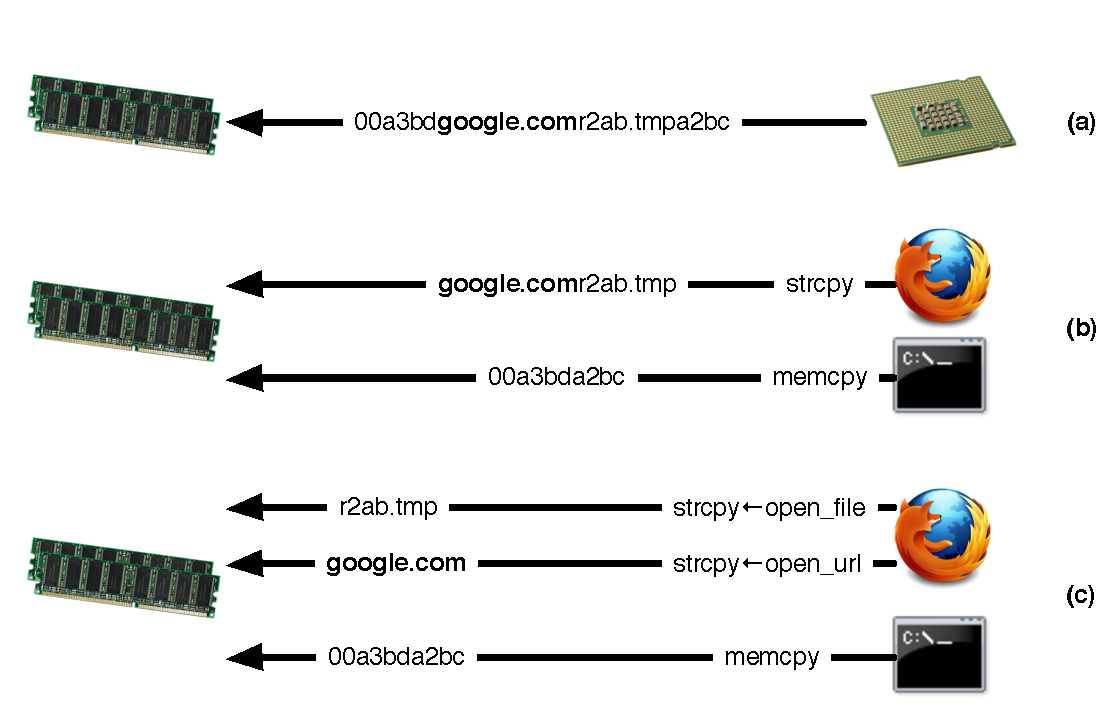
\includegraphics[width=3.2in]{tappoint.pdf}
\end{center}
\caption{Three different ways of defining a tap point: (a) as a single
stream of information from the CPU to RAM ; (b) split up according to
program and location within program ; (c) split up according to program,
location within program, and calling context.}
\label{fig:tappoint}
\end{figure}

A naive approach to defining tap points would be to simply group memory
accesses by the program counter that made them (e.g., EIP/RIP on x86 and
R15 on ARM). However, this approach fails in two common cases: first,
memory accesses made by bulk copy functions, such as \texttt{memcpy} and
\texttt{strcpy}, would all be grouped together, which would commingle
data from different parts of the program into the same tap point. In
addition, looking only at the program counter would conflate accesses
from different programs.

Instead, we define tap points as the triple $(caller, program\_counter,
address\_space)$. Including the caller and the address space (the
\texttt{CR3} register on x86, and the \fixme{register} on ARM) separates
out memory accesses into streams that should, in general contain the
same type of data. Figure \ref{fig:tappoint} shows the effect of
choosing various definitions of a tap point when looking for the place
where the browser writes the URL entered by the user (``google.com'').
At the coarsest granularity (a), one can simply look at all writes from
the CPU to RAM; however, the desired information is buried among reams
of irrelevant data. Separating out tap points by program and program
counter (b) is better, but still combines uses of \texttt{strcpy} that
contain different information --- in this case, a filename and a URL. By
including the calling context (c), we can finally obtain a tap point
that contains just the desired information.

Collecting information about the caller is accomplished in TZB in an
architecture-specific way. On 32-bit x86, we simply read the return
address off the stack. Aside from a small number of functions which are
optimized using frame pointer omission, this reliably gets the call site
for the current function. On other architectures, where stack-walking is
unreliable, we can run a pass that constructs a shadow stack based on
function calls and returns, which allows us to generically obtain an
accurate call stack at all times, but takes extra time up-front to
compute.

Although it is possible that some tap points may require deeper
information about the calling context (for example, if an application
has its own wrapper around \texttt{memcpy}), we have found that just one
level of calling context is usually sufficient. In addition, because TZB
is a whole-system emulator that can watch every call and return, we can
obtain the call stack to an arbitrary depth for any tap point. This
makes it easy to add extra context for a given tap point, if it is found
that doing so separates out the desired information.

\fixme{Might need to cut this paragraph since we haven't tested the tap
point correlation stuff.} Conversely, one might wonder whether this
definition of a tap point may split up data that should logically be
kept together. To address this case, we introduce the idea of
\emph{correlated tap points}: we can run a pass over the recorded
execution that notices when two tap points write to adjacent locations
in memory. The idea is that these tap points may be more usefully
considered jointly; for example, a single data structure may have its
fields set by successive writes. These writes would come from different
program counters, and hence would be split into different tap points,
but it may be more useful to examine the data structure as a whole. By
noticing this correlation we can analyze the data from the combined tap
point.

\subsection{Fully Supervised}



\subsection{Semi-Supervised}

\subsection{Unsupervised}
